
\let\negmedspace\undefined
\let\negthickspace\undefined
\documentclass[journal,12pt,onecolumn]{IEEEtran}
\usepackage{cite}
\usepackage{amsmath,amssymb,amsfonts,amsthm}
\usepackage{algorithmic}
\usepackage{amsmath}
\usepackage{graphicx}
\graphicspath{{./figs/}}
\usepackage{textcomp}
\usepackage{framed} 
\usepackage[utf8]{inputenc}   % for UTF-8 input
\usepackage[T1]{fontenc}      % proper font encoding
\usepackage{lmodern}          % better fonts
\usepackage[utf8]{inputenc}
\usepackage{xcolor}
\usepackage{txfonts}
\usepackage{romannum}
\usepackage{listings}
\usepackage{enumitem}
\usepackage{mathtools}
\usepackage{gensymb}
\usepackage{comment}
\usepackage{caption}
\usepackage[breaklinks=true]{hyperref}
\usepackage{tkz-euclide} 
\usepackage{listings}
\usepackage{gvv}                                        
\usepackage{color}        
\usepackage[utf8]{inputenc}                                     
\usepackage{array}                                            
\usepackage{longtable}         
\usepackage{multicol}                              
\usepackage{calc}                                             
\usepackage{multirow}
\usepackage{multicol}
\usepackage{hhline}                                           
\usepackage{ifthen}                                           
\usepackage{lscape}
\usepackage{tabularx}
\usepackage{array}
\usepackage{float}
\newtheorem{theorem}{Theorem}[section]
\newtheorem{problem}{Problem}
\newtheorem{proposition}{Proposition}[section]
\newtheorem{lemma}{Lemma}[section]
\newtheorem{corollary}[theorem]{Corollary}
\newtheorem{example}{Example}[section]
\newtheorem{definition}[problem]{Definition}
\newcommand{\BEQA}{\begin{eqnarray}}
	\newcommand{\EEQA}{\end{eqnarray}}

\theoremstyle{remark}

\title{\textbf{GATE CS 2015 SET-2}}
\author{ EE25BTECH11052 - Shriyansh Kalpesh Chawda}
\begin{document}
\maketitle
	\fbox{{\Large Q. No. 1 – 5 Carry One Mark Each}}
	\vspace{0.4cm}
	\begin{enumerate}
		
		\item Based on the given statements, select the most appropriate option to solve the given question
		
		What will be the total weight of $10$ poles each of same weight?
		
		Statements: \brak{I} One fourth of the weight of a pole is $15$kg.
		
		\brak{II} The total weight of these poles is $160$ kg more than the total weight of two poles
		
		\hfill{\brak{\text{GATE CS 2015}}}
		
		\begin{enumerate}
			\begin{multicols}{2}
				\item Statement I alone is not sufficient
				\item Statement II alone is not sufficient\\
				\item Either I or II alone is sufficient
				\item Both statements I and II together are not sufficient.
			\end{multicols}
		\end{enumerate}
		
		\item Consider a function
		$f\brak{x} = 1 - |x| \text{ on } -1 < x < 1$
		The value of $x$ at which the function attains a maximum, and the maximum value of the function are.
		
		\hfill{\brak{\text{GATE CS 2015}}}
		
		\begin{enumerate}
			\begin{multicols}{4}
				\item $0$, $-1$
				\item $-1$, $0$
				\item $0$, $1$
				\item $-1$, $2$
			\end{multicols}
		\end{enumerate}
		
		\item A generic term that include various items of clothing such as a skirt, a pair of trousers and a shirt is
		
		\hfill{\brak{\text{GATE CS 2015}}}
		
		\begin{enumerate}
			\begin{multicols}{4}
				\item fabric
				\item textile
				\item fibre
				\item apparel
			\end{multicols}
		\end{enumerate}
		
		\item Choose the statement where underlined word is used correctly.
		
		\hfill{\brak{\text{GATE CS 2015}}}
		
		\begin{enumerate}
			\begin{multicols}{2}


			\item The industrialist load a personnel jet.
			\item I write my experience in my personnel diary.
			\item All personnel are being given the day off.
			\item Being religious is a personnel aspect.
						\end{multicols}
		\end{enumerate}
		
		\item We \underline{\hspace{2cm}} our friend's birthday and we \underline{\hspace{2cm}} how to make it up to him.
		
		\hfill{\brak{\text{GATE CS 2015}}}
		
		\begin{enumerate}
			\begin{multicols}{2}


			\item Completely forgot --- don't just know
			\item Forgot completely --- don't just know
			\item Completely forgot --- just don't know
			\item Forgot completely --- just don't know
						\end{multicols}
		\end{enumerate}
		
		\item In a triangle $PQR$, $PS$ is the angle bisector of $\angle QPR$ and $\angle QPS = 60\degree$.
		\begin{figure}[H]
			\centering
			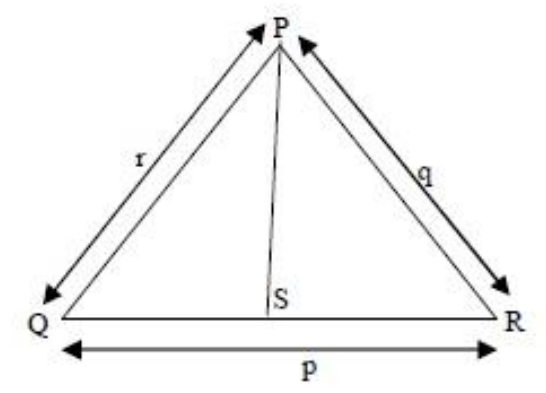
\includegraphics[width=0.3\linewidth]{figs/screenshot001}
			\caption{}
			\label{fig:screenshot001}
		\end{figure}
		

		
		What is the length of $PS$?
		
		\hfill{\brak{\text{GATE CS 2015}}}
		
		\begin{enumerate}
			\begin{multicols}{4}
				\item $\frac{q+r}{qr}$
				\item $\frac{qr}{q+r}$
				\item $\frac{q+r}{2\sqrt{2}}$
				\item $\frac{q+r}{2qr}$
			\end{multicols}
		\end{enumerate}
		
		\item Out of the following four sentences, select the most suitable sentence with respect to grammar and usage.
		
		\hfill{\brak{\text{GATE CS 2015}}}
		
		\begin{enumerate}
			\item Since the report lacked needed information, it was of no use to them.
			\item The report was useless to them because there were no needed information in it.
			\item Since the report did not contain the needed information, it was not real useful to them
			\item Since the report lacked needed information, it would not had been useful to them.
		\end{enumerate}
		
		\item If the list of letters, $P,R,S,T,U$ is an arithmetic sequence, which of the following are also in arithmetic sequence?
		
		I. $2P^2, 2R^2, 2S^2, 2T^2, 2U^2$
		
		II. $P-3,R-3,S-3,T-3, U-3$
		
		III. $P^2, R^2, S^2,T^2, U^2$
		
		\hfill{\brak{\text{GATE CS 2015}}}
		
		\begin{enumerate}
			\begin{multicols}{4}
				\item I only
				\item I and II
				\item II and III
				\item I and III
			\end{multicols}
		\end{enumerate}
		
		\item If $p, q, r, s$ are distinct integers such that:
		$$f\brak{p,q,r,s} = \max\brak{p,q,r,s}$$
		$$g\brak{p,q,r,s} = \min\brak{p,q,r,s}$$
		$$h\brak{p,q,r,s} = \text{remainder of } \frac{p+q}{r+s} \text{ if } \brak{p+q} \geq \brak{r+s}$$
		or remainder of $\frac{r+s}{p+q}$ if $\brak{r+s} > \brak{p+q}$
		
		Also a function $fgh\brak{p,q,r,s} = f\brak{p,q,r,s} \times g\brak{p,q,r,s} \times h\brak{p,q,r,s}$
		
		Also the same operations are valid with two variable functions of the form $f\brak{p,q}$
		
		What is the value of $fg\brak{h\brak{2,5,7,3}, 4,6,8}$?
		
		\hfill{\brak{\text{GATE CS 2015}}}
		
		\item Four branches of a company are located at $M,N,O$ and $P$. $M$ is north of $N$ at a distance of $4$km: $P$ is south of $O$ at a distance of $2$ km: $N$ is southeast of $O$ by $1$ km. What is the distance between $M$ and $P$ in km?
		
		\hfill{\brak{\text{GATE CS 2015}}}
		
		\begin{enumerate}
			\begin{multicols}{4}
				\item $5.34$
				\item $6.74$
				\item $28.5$
				\item $45.49$
			\end{multicols}
		\end{enumerate}
		
	\end{enumerate}
	\newpage
\section*{\Large COMPUTER SCIENCE AND ENGINEERING}
		\vspace{0.5cm}
	\fbox{\large Q. No. 1 - 25 Carry One Mark Each}
	\vspace{0.5cm}
	\begin{enumerate}
		
		\item An unordered list contain $n$ distinct elements. The number of comparisons to find an element in this list that is neither maximum nor minimum is
		
		\hfill{\brak{\text{GATE CS 2015}}}
		
		\begin{enumerate}
			\begin{multicols}{4}
				\item $\Theta\brak{n \log n}$
				\item $\Theta\brak{n}$
				\item $\Theta\brak{\log n}$
				\item $\Theta\brak{1}$
			\end{multicols}
		\end{enumerate}
		
		\item Let $R$ be the relation on the set of positive integers such that $aRb$ if and only if $a$ and $b$ are distinct and have a common divisor other than $1$. Which one of the following statements about $R$ is true?
		
		\hfill{\brak{\text{GATE CS 2015}}}
		
		\begin{enumerate}
			\item $R$ is symmetric and reflexive but not transitive
			\item $R$ is reflexive but not symmetric and not transitive
			\item $R$ is transitive but not reflexive and not symmetric
			\item $R$ is symmetric but not reflexive and not transitive
		\end{enumerate}
		
		\item Consider the following transaction involving two bank account $x$ and $y$.
		
		read $\brak{x}$ ; $x \colon= x - 50$; write $\brak{x}$ ; read $\brak{y}$; $y \colon= y + 50$ ; write $\brak{y}$
		
		The constraint that the sum of the accounts $x$ and $y$ should remain constant is that of
		
		\hfill{\brak{\text{GATE CS 2015}}}
		
		\begin{enumerate}
			\begin{multicols}{4}
				\item Atomicity
				\item Consistency
				\item Isolation
				\item Durability
			\end{multicols}
		\end{enumerate}
		
		\item A binary tree $T$ has $20$ leaves. The number of nodes in $T$ having two children is \underline{\hspace{2cm}}.
		
		\hfill{\brak{\text{GATE CS 2015}}}
		
		\item Consider the basic COCOMO model where $E$ is the effort applied in person-months, $D$ is the development time in chronological months, KLOC is the estimated number of delivered lines of code \brak{in thousands} and $a_b,b_b, c_b,d_b$ have their usual meanings. The basic COCOMO equations are of the form
		
		\hfill{\brak{\text{GATE CS 2015}}}
		
		\begin{enumerate}
			\begin{multicols}{2}
			\item $E = a_b\brak{\text{KLOC}}^{\exp\brak{b_b}},D = c_b\brak{E}^{\exp\brak{d_b}}$
			\item $D = a_b\brak{\text{KLOC}}^{\exp\brak{b_b}},E = c_b\brak{D}^{\exp\brak{d_b}}$
			\item $E = a_b^{\exp\brak{b_b}},D = c_b\brak{\text{KLOC}}^{\exp\brak{d_b}}$
			\item $E = a_b^{\exp\brak{D}},D = c_b\brak{\text{KLOC}}^{\exp\brak{b_b}}$
						\end{multicols}
		\end{enumerate}
		
		\item Consider the following two statements.
		
		$S_1$: If a candidate is known to be corrupt, then he will not be elected
		
		$S_2$: If a candidate is kind, he will be elected
		
		Which one of the following statements follows from $S_1$ and $S_2$ per sound inference rules of logic?
		
		\hfill{\brak{\text{GATE CS 2015}}}
		
		\begin{enumerate}
			\item If a person is known to corrupt, he is kind
			\item If a person is not known to be corrupt, he is not kind
			\item If a person is kind, he is not known to be corrupt
			\item If a person is not kind, he is not known to be corrupt
		\end{enumerate}
		
		\item Assume that for a certain processor, a read request takes $50$ nanoseconds on a cache miss and $5$ nanoseconds on a cache hit. Suppose while running a program, it was observed that $80\%$ of the processors read requests result in a cache hit. The average and access time in nanoseconds is \underline{\hspace{2cm}}.
		
		\hfill{\brak{\text{GATE CS 2015}}}
		
		\item A system has $6$ identical resources and $N$ processes competing for them. Each process can request atmost $2$ resources. Which one of the following values of $N$ could lead to a deadlock?
		
		\hfill{\brak{\text{GATE CS 2015}}}
		
		\begin{enumerate}
			\begin{multicols}{4}
				\item $1$
				\item $2$
				\item $3$
				\item $4$
			\end{multicols}
		\end{enumerate}
		
		\item Consider a complete binary tree where the left and the right subtrees of the root are max-heaps. The lower bound for the number of operations to convert the tree to a heap is
		
		\hfill{\brak{\text{GATE CS 2015}}}
		
		\begin{enumerate}
			\begin{multicols}{4}
				\item $\Theta\brak{\log n}$
				\item $\Theta\brak{n}$
				\item $\Theta\brak{n \log n}$
				\item $\Theta\brak{n^2}$
			\end{multicols}
		\end{enumerate}
		
		\item In the context of abstract-syntax-tree \brak{AST} and control-flow-graph \brak{CFG}, which one of the following is TRUE?
		
		\hfill{\brak{\text{GATE CS 2015}}}
		
		\begin{enumerate}
			\item In both AST and CFG, let node, $N_2$ be the successor of node $N_1$. In the input program, the code corresponding to $N_2$ is present after the code corresponding in $N_1$.
			\item For any input program, neither AST nor CFG will contain a cycle
			\item The maximum number of successors of a node in an AST and a CFG depends on the input program
			\item Each node is AST and CFG corresponds to at most one statement in the input program
		\end{enumerate}
		
		\item With reference to the B+ tree index of order $1$ shown below, the minimum number of nodes \brak{including the Root node} that must be fetched in order to satisfy the following query: "Get all records with a search key greater than or equal to $7$ and less than $15$" is \underline{\hspace{2cm}}
		
\begin{figure}[H]
	\centering
	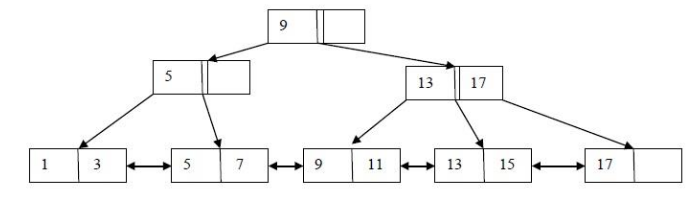
\includegraphics[width=0.7\linewidth]{figs/screenshot002}
	\caption{}
	\label{fig:screenshot002}
\end{figure}

		
		\hfill{\brak{\text{GATE CS 2015}}}
		
		\item A software requirements specification \brak{SRS} document should avoid discussing which one of the following?
		
		\hfill{\brak{\text{GATE CS 2015}}}
		
		\begin{enumerate}
			\begin{multicols}{2}
				\item User interface issues
				\item Non-functional requirements
				\item Design specification
				\item Interfaces with third party software
			\end{multicols}
		\end{enumerate}
		
		\item Identify the correct order in which a server process must invoke the function calls accept, bind, listen, and recv according to UNIX socket APL
		
		\hfill{\brak{\text{GATE CS 2015}}}
		
		\begin{enumerate}
\begin{multicols}{2}


\item listen, accept, bind recv
			\item bind, listen, accept, recv
			\item bind, accept, listen, recv
			\item accept, listen, bind recv
\end{multicols}
		\end{enumerate}
		
		\item The larger of the two eigen values of the matrix $\myvec{4 & 5 \\ 2 & 1}$ is \underline{\hspace{2cm}}
		
		\hfill{\brak{\text{GATE CS 2015}}}
		
		\item The cardinality of the power set of $\brak{0, 1, 2,......10}$ is \underline{\hspace{2cm}}
		
		\hfill{\brak{\text{GATE CS 2015}}}
		
		\item Which one of the following statements is NOT correct about HTTP cookies?
		
		\hfill{\brak{\text{GATE CS 2015}}}
		
		\begin{enumerate}
			\item A cookie is a piece of code that has the potential to compromise the security of an internet user
			\item A cookie gains entry to the user's work area through an HTTP header
			\item A cookie has an expiry date and time
			\item Cookies can be used to track the browsing pattern of a user at a particular site
		\end{enumerate}
		
		\item Consider the following function written the C programming language.
		\begin{align*}
			&\text{void foo}\brak{\text{char * a}} \{\\
			&\text{if } \brak{*a \text{ \&\& } *a != '\text{ }'} \{\\
			&\text{putchar}\brak{*a};\\
			&\}\\
			&\}
		\end{align*}
		
		The output of the above function on input "ABCD EFGH" is
		
		\hfill{\brak{\text{GATE CS 2015}}}
		
		\begin{enumerate}
			\begin{multicols}{4}
				\item ABCD EFGH
				\item ABCD
				\item HGFE DCBA
				\item DCBA
			\end{multicols}
		\end{enumerate}
		
		\item A link has a transmission speed of $10^6$ bits/sec. It uses data packets of size $1000$ bytes each. Assume that the acknowledgement has negligible transmission delay, and that its propagation delay is the same as the data propagation delay. Also assume that the processing delays at the nodes are negligible. The efficiency of the stop-and-wait protocol in this setup is exactly $25\%$. The value of the one-way propagation delay \brak{in  milliseconds} is \underline{\hspace{2cm}}.
		
		\hfill{\brak{\text{GATE CS 2015}}}
		
		\item The minimum number of JK flip-flops required to construct a synchronous counter with the count sequence $\brak{0,0, 1, 1, 2, 2, 3, 3, 0, 0,......}$ is \underline{\hspace{2cm}}.
		
		\hfill{\brak{\text{GATE CS 2015}}}
		
		\item Match the following:
		\begin{figure}[H]
			\centering
			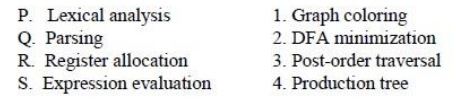
\includegraphics[width=0.6\linewidth]{figs/screenshot003}
		\end{figure}
		
		\hfill{\brak{\text{GATE CS 2015}}}
		
		\begin{enumerate}
			\begin{multicols}{2}
				\item $P-2, Q-3, R-1, S-4$
				\item $P-2, Q-1, R-4, S-3$
				\item $P-2, Q-4, R-1, S-3$
				\item $P-2, Q-3, R-4, S-1$
			\end{multicols}
		\end{enumerate}
		
		\item Consider two decision problems $Q_1$, $Q_2$ such that $Q_1$ reduces in polynomial time to $3$-SAT and $3$-SAT reduces in polynomial time to $Q_2$. Then which one of following is consistent with the above statement?
		\hfill{\brak{\text{GATE CS 2015}}}
		
		\begin{enumerate}
			\begin{multicols}{2}


			\item $Q_1$ is in NP, $Q_2$ in NP hard
			\item $Q_2$ is in NP, $Q_1$ is NP hard
			\item Both $Q_1$ and $Q_2$ are in NP
			\item Both $Q_1$ and $Q_2$ are NP hard
						\end{multicols}
		\end{enumerate}
		
		\item A computer system implements a $40$-bit virtual address, page size of $8$ kilobytes, and a $128$-entry translation look-aside buffer \brak{TLB} organized into $32$ sets each having four ways. Assume that the TLB tag does not store any process id. The minimum length of the TLB tag in bits is \underline{\hspace{2cm}}.
		
		\hfill{\brak{\text{GATE CS 2015}}}
		
		\item Consider the following C function.
		
\begin{verbatim}
			int fun (int n) 
			int x = 1, k;
			if  (n == 1)  return x};
			for  (k = 1; k < n; k++)
			x = x + fun(k) * fun(n - k);
		return x;
			}
\end{verbatim}

		The return value of fun $\brak{5}$ is \underline{\hspace{2cm}}
		
		\hfill{\brak{\text{GATE CS 2015}}}
		
		\item Consider the following statements
		
		I. The complement of every Turing decidable language is Turing decidable
		
		II. There exists some language which is in NP but is not turing decidable
		
		III. If $L$ is a language in NP, $L$ is turing decidable
		
		Which of the above statements is/are true?
		
		\hfill{\brak{\text{GATE CS 2015}}}
		
		\begin{enumerate}
			\begin{multicols}{4}
				\item Only II
				\item Only III
				\item Only I and II
				\item Only I and III
			\end{multicols}
		\end{enumerate}
		
		\item The number of divisors of $2100$ is \underline{\hspace{2cm}}.
		
		\hfill{\brak{\text{GATE CS 2015}}}\\
		\fbox{\large Q.No-26-55 Carry Two Marks Each}
		\vspace{.6cm}
		
		\item In a connected graph, a bridge is an edge whose removal disconnects a graph. Which one of the following statements is true?
		
		\hfill{\brak{\text{GATE CS 2015}}}
		
		\begin{enumerate}
			\item A tree has no bridges
			\item A bridge cannot be part of a simple cycle
			\item Every edge of a clique with size $\geq 3$ is a bridge \brak{A clique is any compete sub graph of a graph}
			\item A graph with bridges cannot have a cycle
		\end{enumerate}
		
		\item Consider six memory partitions of sizes $200$ KB, $400$ KB, $600$ KB, $500$ KB, $300$ KB and $250$ KB, where KB refers to kilobyte. These partitions need to be allotted to four processes of sizes $357$ KB, $210$KB, $468$ KB and $491$ KB in that order. If the best fit algorithm is used, which partitions are NOT allotted to any process?
		
		\hfill{\brak{\text{GATE CS 2015}}}
		
		\begin{enumerate}
			\begin{multicols}{4}
				\item $200$KB and $300$ KB
				\item $200$KB and $250$ KB
				\item $250$KB and $300$ KB
				\item $300$KB and $400$ KB
			\end{multicols}
		\end{enumerate}
		
		\item Which one of the following assertions concerning code inspection and code walkthrough is true?
		
		\hfill{\brak{\text{GATE CS 2015}}}
		
		\begin{enumerate}
			\item Code inspection is carried out once the code has been unit tested
			\item Code inspection and code walkthrough are synonyms
			\item Adherence to coding standards is checked during code inspection
			\item Code walkthrough is usually carried out by an independent test team
		\end{enumerate}
		
		\item Given below are some algorithms, and some algorithm design paradigms.\\
		\vspace{0.6cm}
		
		\begin{tabular}{|l|l|}
			\hline
			(1) Dijkstra’s Shortest Path & (i) Divide and Conquer \\
			\hline
			(2) Floyd-Warshall algorithm to compute all pair shortest path & (ii) Dynamic Programming \\
			\hline
			(3) Binary search on a sorted array & (iii) Greedy design \\
			\hline
			(4) Backtracking search on a graph & (iv) Depth-first search \\
			\hline
			& (v) Breadth-first search \\
			\hline
		\end{tabular}
				\vspace{0.6cm}

		
		Match the above algorithms on the left to the corresponding design paradigm they follow.
		
		\hfill{\brak{\text{GATE CS 2015}}}
		
		\begin{enumerate}
			\begin{multicols}{2}
				\item $1-i, 2-iii, 3-i, 4-v$
				\item $1-iii, 2-iii, 3-i, 4-v$
				\item $1-iii, 2-ii, 3-i, 4-iv$
				\item $1-iii, 2-ii, 3-i, 4-v$
			\end{multicols}
		\end{enumerate}
		
		\item Suppose you are provided with the following function declaration in the C programming language
		
		int partition $\brak{\text{int a } [ ], \text{int n}}$;
		
		The function treats the first element of a $[ ]$ as a pivot, and rearranges the array so that all elements less than or equal to the pivot is in the left part of the array, and all elements greater than the pivot is in the right part. In addition, it moves the pivot so that the pivot is the last elements of the left part. The return value is the number of elements in the left part.
		
		The following partially given function in the C programming language is used to find the $K$th smallest element in an array a $[ ]$ of size $n$ using the partition function We assume $k \leq n$.
		
	\begin{verbatim}
		int kth_smallest(int a, int n, int k)
		{
			int left_end = partition(a, n);
			if (left_end + 1 == k) {
				return a[left_end];
			}
			if (left_end + 1 > k) {
				return kth_smallest(__________________);
			} else {
				return kth_smallest(__________________________);
			}
		}
	\end{verbatim}
		
		The missing argument lists are respectively
		
		\hfill{\brak{\text{GATE CS 2015}}}
		
		\begin{enumerate}
			\item $\text{a, left\_end,k}$ and $\text{a} + \text{left\_end} + 1, \text{n} - \text{left\_end} - 1, \text{k} - \text{left\_end} - 1$
			\item $\text{a, left\_end,k}$ and $\text{a, n} - \text{left\_end} - 1, \text{k} - \text{left\_end} - 1$
			\item $\text{a} + \text{left\_end} + 1,\text{n} - \text{left\_end} - 1, \text{k} - \text{left\_end} - 1$ and $\text{a, left\_end, k}$
			\item $\text{a, n} - \text{left\_end} - 1, \text{k} - \text{left\_end} - 1$ and $\text{a, left\_end,k}$
		\end{enumerate}
		
		\item Consider a typical disk that rotates at $15000$ rotations per minute \brak{RPM} and has a transfer rate of $50 \times 10^6$ bytes/sec. if the average seek time of the disk is twice the average rotational delay and the controller's transfer time is $10$ times the disk transfer time, the average time \brak{in milliseconds} to read or write a $512$-byte sector of the disk is \underline{\hspace{2cm}}.
		
		\hfill{\brak{\text{GATE CS 2015}}}
		
		\item Let $f\brak{x} = \frac{1}{x^3}$ and $A$ denote the area of the region bounded by $f\brak{x}$ and the X-axis, when $x$ varies from $-1$ to $1$. Which of the following statements is/are TRUE?
		
		\brak{I} $f$ is continuous in $\brak{-1,1}$
		
		\brak{II} $f$ is not bounded in $\brak{-1,1}$
		
		\brak{III} $A$ is nonzero and finite
		
		\hfill{\brak{\text{GATE CS 2015}}}
		
		\begin{enumerate}
			\begin{multicols}{4}
				\item II only
				\item III only
				\item II and III only
				\item I, II and III
			\end{multicols}
		\end{enumerate}
		
		\item Consider the intermediate code given below.
		\begin{align*}
			&\brak{1} \quad i = 1\\
			&\brak{2} \quad j = 1\\
			&\brak{3} \quad t1 = 5 * i\\
			&\brak{4} \quad t2 = t1 + j\\
			&\brak{5} \quad t3 = 4 * t2\\
			&\brak{6} \quad t4 = t3\\
			&\brak{7} \quad a[t4] = 1\\
			&\brak{8} \quad j = j + 1\\
			&\brak{9} \quad \text{if } j \leq 5 \text{ goto } 3\\
			&\brak{10} \quad i = i + 1\\
			&\brak{11} \quad \text{if } i \leq 5 \text{ goto } 2
		\end{align*}
		
		The number of nodes and edges in the control-flow-graph constructed for the above code, respectively, are
		
		\hfill{\brak{\text{GATE CS 2015}}}
		
		\begin{enumerate}
			\begin{multicols}{4}
				\item $5$ and $7$
				\item $6$ and $7$
				\item $5$ and $5$
				\item $7$ and $8$
			\end{multicols}
		\end{enumerate}
		
		\item The number of min-terms after minimizing the following Boolean expression is \underline{\hspace{2cm}}.
		
		$D' + AB' + A'C + AC'D + A'C'D'$
		
		\hfill{\brak{\text{GATE CS 2015}}}
		
		\item The number of onto function \brak{surjective functions} from set $X = \{1,2,3,4\}$ to set $Y = \{a,b,c\}$ is \underline{\hspace{2cm}}.
		
		\hfill{\brak{\text{GATE CS 2015}}}
		
		\item Consider the alphabet $\Sigma = \{0,1\}$, the null/empty string $\epsilon$ and the sets of strings $X_0$, $X_1$, and $X_2$ generated by the corresponding non-terminals of regular grammar. $X_0$, $X_1$, and $X_2$ are related as follows:
		\begin{align*}
			X_0 &= 1X_1\\
			X_1 &= 0X_1 + 1X_2\\
			X_2 &= 0X_1 + \epsilon
		\end{align*}
		
		Which one of the following choices precisely represents the strings in $X_0$?
		
		\hfill{\brak{\text{GATE CS 2015}}}
		
		\begin{enumerate}
			\begin{multicols}{2}


			\item $1\brak{0 + 10}^*\brak{10}^* + 1$
			\item $1\brak{0 + 10}^*\brak{10}^* *1$
			\item $1\brak{0 + 10}^*1$
			\item $1\brak{0 + 10}^*1 + 11\brak{0 + 10}^*1$
						\end{multicols}
		\end{enumerate}
		
		\item Which of the following languages is/are regular?
		
		$L_1 = \{wxw^R \mid w, x \in \{a, b\}^* \text{ and } |w| \geq 0 , |x| \geq 0, w^R \text{ is the reverse of string } w\}$
		
		$L_2 = \{a^n b^m \mid m \neq n \text{ and } m, n \geq 0\}$
		
		$L_3 = \{a^p b^q c^r \mid p,q, r \geq 0\}$
		
		\hfill{\brak{\text{GATE CS 2015}}}
		
		\begin{enumerate}
			\begin{multicols}{4}
				\item $L_1$ and $L_3$ only
				\item $L_1$ only
				\item $L_2$ and $L_3$ only
				\item $L_3$ only
			\end{multicols}
		\end{enumerate}
		
		\item Consider a processor with byte-addressable memory. Assume that all registers, including Program Counter \brak{PC} and Program Status Word \brak{PSW}, are of size $2$ bytes. A stack in the main memory is implemented from memory location $\brak{0100}_{16}$ and it grows upward. The stack pointer \brak{SP} points to the top element of the stack. The current value of SP is $\brak{016E}_{16}$. The CALL instruction is of two words, the first word is the op-code and the second word is the starting address of the subroutine. \brak{one word = 2bytes}. The CALL instruction is implemented as follows:
		
		\begin{itemize}
			\item Store the current Vale of PC in the Stack
			\item Store the value of PSW register in the stack
			\item Load the starting address of the subroutine in PC
		\end{itemize}
		
		The content of PC just before the fetch of a CALL instruction is $\brak{5FA0}_{16}$. After execution of the CALL instruction, the value of the stack pointer is
		
		\hfill{\brak{\text{GATE CS 2015}}}
		
		\begin{enumerate}
			\begin{multicols}{4}
				\item $\brak{016A}_{16}$
				\item $\brak{016C}_{16}$
				\item $\brak{0170}_{16}$
				\item $\brak{0172}_{16}$
			\end{multicols}
		\end{enumerate}
		
		\item The number of states in the minimal deterministic finite automaton corresponding to the regular expression $\brak{0 + 1}^* \brak{10}$ is \underline{\hspace{2cm}}
		
		\hfill{\brak{\text{GATE CS 2015}}}
		
		\item Host A sends a UDP datagram containing $8880$ bytes of user data to host B over an Ethernet LAN. Ethernet frames may carry data up to $1500$ bytes \brak{i.e. MTU = 1500 bytes}. Size of UDP header is $8$ bytes and size of IP heard is $20$ bytes. There is no option field in IP header How many total number of IP fragments will be transmitted and what will be the contents of offset field in the last fragment?
		
		\hfill{\brak{\text{GATE CS 2015}}}
		
		\begin{enumerate}
			\begin{multicols}{4}
				\item $6$ and $95$
				\item $6$ and $7400$
				\item $7$ and $1110$
				\item $7$ and $8880$
			\end{multicols}
		\end{enumerate}
		
		\item Consider the following routing table at an IP router:
		
		\begin{table}[h]
			\centering
			\begin{tabular}{|c|c|c|}
				\hline
				Network No. & Net Mask & Next Hop \\
				\hline
				128.96.170.0 & 255.255.254.0 & Interface 0 \\
								\hline				
				128.96.168.0 & 255.255.254.0 & Interface 1 \\
								\hline
				128.96.166.0 & 255.255.254.0 & R2 \\
								\hline
				128.96.164.0 & 255.255.252.0 & R3 \\
								\hline
				0.0.0.0 & Default & R4 \\
				\hline
			\end{tabular}
		\end{table}
		
		For each IP address in Group I identify the correct choice of the next hop from Group II using the entries from the routing table above.
		
		\begin{table}[H]
			\centering
			\begin{tabular}{|c|c|}
				\hline
				Group I & Group II \\
				\hline
				\brak{i} 128.96.171.92 & \brak{a} Interface 0 \\
				\hline
				\brak{ii} 128.96.167.151 & \brak{b} Interface 1 \\
				\hline
				\brak{iii} 128.96.163..151 & \brak{c} R2 \\
				\hline
				\brak{iv} 128.96.165.121 & \brak{d} R3 \\
				\hline
				& \brak{e} R4 \\
				\hline
			\end{tabular}
		\end{table}
		
		\hfill{\brak{\text{GATE CS 2015}}}
		
		\begin{enumerate}
			\begin{multicols}{2}
				\item $i-a, ii-c, iii-e, iv-d$
				\item $i-a, ii-d, iii-b, iv-e$
				\item $i-b, ii-c, iii-d, iv-e$
				\item $i-b, ii-c, iii-e, iv-d$
			\end{multicols}
		\end{enumerate}
		
		\item Consider two relations $R_1\brak{A,B}$ with the tuples $\brak{1.5}, \brak{3,7}$ and $R_2\brak{A,C} = \brak{1,7}, \brak{4,9}$. Assume that $R\brak{A,B,C}$ is the full natural outer join of $R_1$ and $R_2$. Consider the following tuples of the form $\brak{A,B,C}$: 
		$a = \brak{1.5, \text{null}}$, $b = \brak{1, \text{null},7}$, $c = \brak{3, \text{null},9}$, $d = \brak{4,7,\text{null}}$, $e = \brak{1,5,7}$, $f = \brak{3,7, \text{null}}$, $g = \brak{4, \text{null},9}$.
		
		Which one of the following statements is correct?
		
		\hfill{\brak{\text{GATE CS 2015}}}
		
		\begin{enumerate}\begin{multicols}{2}


			\item $R$ contains $a, b, e, f, g$ but not $c, d$.
			\item $R$ contains all of $a, b, c, d, e, f, g$
			\item $R$ contains $e, f, g$ but not $a, b$
			\item $R$ contains $e$ but not $f, g$
						\end{multicols}
		\end{enumerate}
		
		\item Consider a simple check pointing protocol and the following set of operations in the log.
		
		$\brak{\text{Start}, T_4}; \brak{\text{write}, T_4, y,2,3}; \brak{\text{Start}, T_1}; \brak{\text{commit},T_4}; \brak{\text{write}, T_1,z,5,7};$
		
		$\brak{\text{checkpoint}};$
		
		$\brak{\text{Start},T_2}; \brak{\text{write}, T_2, x,1,9}; \brak{\text{commit},T_2}; \brak{\text{start},T_3}, \brak{\text{write},T_3,z,7,2};$
		
		If a crash happens now and the system tries to recover using both undo and redo operations, what are the contents of the undo lists and the redo list?
		
		\hfill{\brak{\text{GATE CS 2015}}}
		
		\begin{enumerate}
					\begin{multicols}{2}
			\item Undo: $T_3,T_1$; Redo: $T_2$
			\item Undo: $T_3,T_1$; Redo: $T_2,T_4$
			\item Undo: none; redo: $T_2,T_4,T_3,T_1$
			\item Undo: $T_3,T_1, T_4$; Redo: $T_2$
									\end{multicols}
		\end{enumerate}
		
		\item A computer system implements $8$ kilobyte pages and a $+32$-bit physical address space. Each page table entry contains a valid bit, a dirty bit, three permission bits, and the translation. If the maximum size of the page table of a process is $24$ megabytes, the length of the virtual address supported by the system is \underline{\hspace{2cm}} bits.
		
		\hfill{\brak{\text{GATE CS 2015}}}
		
		\item Which one of the following hash functions on integers will distribute keys most uniformly over $10$ buckets numbered $0$ to $9$ for $i$ ranging from $0$ to $2020$?
		
		\hfill{\brak{\text{GATE CS 2015}}}
		
		\begin{enumerate}
								\begin{multicols}{2}
			\item $h\brak{i} = i^2 \bmod 10$
			\item $h\brak{i} = i^3 \bmod 10$
			\item $h\brak{i} = \brak{11*i}^2 \bmod 10$
			\item $h\brak{i} = \brak{12*i} \bmod 10$
									\end{multicols}
		\end{enumerate}
		
		\item Assume that the bandwidth for a TCP connection is $1048560$ bits/sec. Let $\alpha$ be the value of RTT in milliseconds. \brak{rounded off to the nearest integer} after which the TCP window scale option is needed. Let $\beta$ be the maximum possible window size the window scale option. Then the values of $\alpha$ and $\beta$ are
		
		\hfill{\brak{\text{GATE CS 2015}}}
		
		\begin{enumerate}
			\item $\alpha = 63$ milliseconds, $\beta = 65535 \times 2^{14}$
			\item $\alpha = 63$ milliseconds, $\beta = 65535 \times 2^{16}$
			\item $\alpha = 500$ milliseconds, $\beta = 65535 \times 2^{14}$
			\item $\alpha = 500$ milliseconds, $\beta = 65535 \times 2^{16}$
		\end{enumerate}
		
		\item A young tableau is a 2D array of integers increasing from left to right and from top to bottom. Any unfilled entries are marked with $\infty$, and hence there cannot be any entry to the right of $\infty$, or below a $\infty$.
		
		The following Young tableau consists of unique entries.


\begin{center}
	\setlength{\arrayrulewidth}{0.8pt}
	\renewcommand{\arraystretch}{1.5}
	
	\begin{tabular}{|c|c|c|c|}
		\hline
		1  & 2  & 5  & 14 \\
		\hline
		3  & 4  & 6  & 23 \\
		\hline
		10 & 12 & 18 & 25 \\
		\hline
		31 & $\infty$ & $\infty$ & $\infty$ \\
		\hline
	\end{tabular}
\end{center}
When an element is removed from a Young tableau, other elements should be moved into its place so that the resulting table is still a Young tableau $\brak{unfilled entries may be filled in with a \infty}$. The minimum number of entries $\brak{other than 1}$ to be shifted, to remove $1$ from the given Young tableau is \underline{\hspace{2cm}}
		
		\hfill{\brak{\text{GATE CS 2015}}}
		
		\item A half adder is implemented with XOR and AND gates. A full adder is implemented with two half adders and one OR gate. The propagation delay of an XOR gate is twice that of an AND/OR gate. The propagation delay of an AND/OR gate is $1.2$ microseconds. A $4$-bit ripple-carry binary adder is implemented by using four full adders. The total propagation time of this $4$-bit binary adder in microseconds is \underline{\hspace{2cm}}.
		
		\hfill{\brak{\text{GATE CS 2015}}}
		
		\item Consider the sequence of machine instruction given below:
		
		MUL $R_5, R_0, R_1$
		
		DIV $R_6, R_2, R_3$
		
		ADD $R_7, R_5, R_6$
		
		SUB $R_8, R_7, R_4$
		
		In the above sequence, $R_0$ to $R_8$ are general purpose registers. In the instructions shown. the first register stores the result of the operation performed on the second and the third registers. This sequence of instructions is to be executed in a pipelined instruction processor with the following $4$ stages \brak{1} Instruction Fetch and Decode \brak{IF}, \brak{2} Operand Fetch \brak{OF}, \brak{3} Perform Operation \brak{PO} and \brak{4} Write back the result \brak{WB} . The IF,OF and WB stages take $1$ clock cycle each for any instruction The PO stage takes $1$ clock cycle for ADD or SUB instruction, $3$ clock cycles for MUL instruction and $5$ clock cycles for DIV instruction. The pipelined processor uses operand forwarding from the PO stage to the OF stage. The number of clock cycles taken for the execution of the above sequence of instructions is \underline{\hspace{2cm}}.
		
		\hfill{\brak{\text{GATE CS 2015}}}
		
		\item Perform the following operations on the matrix $\myvec{3 & 4 & 45 \\ 7 & 9 & 105 \\ 13 & 2 & 195}$.
		
		\brak{i} Add the third row to the second row
		
		\brak{ii} Subtract the third column from the first column.
		
		The determinant of the resultant matrix is \underline{\hspace{2cm}}.
		
		\hfill{\brak{\text{GATE CS 2015}}}
		
		\item Which one of the following well formed formulae is a tautology?
		
		\hfill{\brak{\text{GATE CS 2015}}}
		
		\begin{enumerate}
			\item $\forall x \exists y R\brak{x, y} \rightarrow \exists y \forall x R\brak{x, y}$
			\item $\brak{\forall x \exists y \brak{R\brak{x, y} \rightarrow S\brak{x, y}}} \rightarrow \brak{\forall x \exists yS\brak{x, y}}$
			\item $\brak{\forall x \exists y\brak{p\brak{x, y} \rightarrow R\brak{x, y}}} \rightarrow \brak{\forall x \exists y\brak{ P\brak{x, y}} \rightarrow \forall x \exists y R\brak{x, y}}$
			\item $\forall x \exists y p\brak{x, y} \leftrightarrow \forall x \exists y p\brak{y, x}$
		\end{enumerate}
		
		\item A graph is self-complementary if it is isomorphic to its complement For all self-complementary graphs on $n$ vertices, $n$ is
		
		\hfill{\brak{\text{GATE CS 2015}}}
		
		\begin{enumerate}
			\begin{multicols}{2}
				\item A multiple of $4$
				\item Even
				\item Odd
				\item Congruent to $0 \bmod 4$, or, $1 \bmod 4$
			\end{multicols}
		\end{enumerate}
		
		\item The secant method is used to find the root of an equation $f\brak{x} = 0$ . It is started from two distinct estimates, $x_a$ and $x_b$ for the root. It is an iterative procedure involving linear interpolation to a root. The iteration stops if $f\brak{x_b}$ is very small and then $x_b$ is the solution. The procedure is given below. Observe that there is an expression which is missing and is marked by ? Which is the suitable expression that is to be put in place of ? so that it follows all steps of the secant method?
		\begin{verbatim}
Secant
Initialize: xa, xb, e, N        // e = convergence indicator
// N = maximum no. of iterations
fb = f(xb)
i = 0
while (i < N and |fb| > e) do
i = i + 1              // update counter
xt = ?                 // missing expression for xt
xa = xb                // reset xa
xb = xt                // reset xb
fb = f(xb)             // function value at new xb
end while

if |fb| >= e then
write "Non-convergence"     // loop terminated with i = N
else
write "return xb"
End if
		\end{verbatim}
		
		\hfill{\brak{\text{GATE CS 2015}}}
		
		\begin{enumerate}
			\begin{multicols}{2}


			\item $x_b - \frac{f_b\brak{x_b - x_a}}{f_b - f_a}$
			\item $x_a - \frac{f_a\brak{x_a - x_b}}{f_a - f_b}$
			\item $x_b - \frac{\brak{x_b - x_a}}{f_b - f_a} \times f_b$
			\item $x_a - \frac{\brak{x_a - x_b}}{f_a - f_b} \times f_a$
						\end{multicols}
		\end{enumerate}
		
		\item Let $X$ and $Y$ denote the sets containing $2$and $20$ distinct objects respectively and $F$ denote the set of all possible functions defined from $X$ to $Y$. let $f$ be randomly chosen from $F$ .The probability of $f$ being one-to-one is \underline{\hspace{2cm}}.
		
		\hfill{\brak{\text{GATE CS 2015}}}
		
		\item Consider the C program below.
		\begin{verbatim}
#include <stdio.h>
int *A, stkTop;
int stkFunc(int opcode, int val)
{
	static int size = 0, stkTop = 0;
	switch (opcode)
	{
		case -1 : size = val; break;
		case 0  : if (stkTop < size) A[stkTop++] = val; break;
		default : if (stkTop) return A[--stkTop];
	}
	return -1;
}

int main()
{
	int B[20];
	A = B;
	stkTop = -1;
	
	stkFunc(-1, 10);
	stkFunc(0, 5);
	stkFunc(0, 10);
	
	printf("%d\n", stkFunc(1, 0) + stkFunc(1, 0));
}
				\end{verbatim}	
		The value printed by the above program is \underline{\hspace{2cm}}.
		
		\hfill{\brak{\text{GATE CS 2015}}}
		
	\end{enumerate}
	
\end{document}